\section{Runtime Systems}\label{sec:Runtime_Systems}
Before we start discussing \nameref{sec:Code_Generation}, we should look at what the end result of our generation should be.

\begin{remark*}
  It is important to note that \textit{function}, \textit{method}, and \textit{procedure} may be used interchangeably.
  While they are all technically different, for our case here, they all act the same.
  They are just named blocks of code that may take in some additional arguments that act as if they were local variables.
  \textbf{In this case, pass-by-reference and pointers are not handled, discussed, or supported in any way!}
\end{remark*}

There are 2 different portions of code:
\begin{enumerate}[noitemsep]
\item A Read-Only portion
  \begin{itemize}[noitemsep]
  \item The read-only portion is called the ``text'' of the program.
  \item This is the actual code in the program.
  \end{itemize}
\item A Read/Write portion
  \begin{itemize}[noitemsep]
  \item This is the ``data'' portion of the program.
  \item Global variables are here.
    \begin{itemize}[noitemsep]
    \item Global in this sense means global to \emph{this} program, not global to \textbf{all} programs.
    \end{itemize}
  \item The \nameref{def:Heap} is here
  \item The \nameref{def:Call_Stack} is here
  \item The \nameref{def:Class_Descriptor} (If the programming language supports object-oriented programming).
  \end{itemize}
\end{enumerate}

\begin{definition}[Heap]\label{def:Heap}
  The \emph{heap} is a memory organization construct that helps visualize the way memory is used during the execution of a program.
  It is \textbf{\emph{SIGNIFICANTLY}} larger than the \nameref{def:Call_Stack}.

  In an object-oriented language, this is where instances of classes exist.
  These objects are allocated on a first-come first-serve basis.
  When the object is allocated, the amount of memory that the object requires is allocated \textbf{\emph{in a continuous block}}.
  The problem is that if the heap has been extensively used, then there might be enough total memory required to allocate an object, but because it is not in a continuous block, the object cannot be allocated.
  
  This makes deallocation more complex, because when they are deallocated, the program might still view the memory as in-use.
  Additionally, because of the continuous block allocation nature of the heap, it must be organized every once in a while.
  This is called \nameref{def:Garbage_Collection}.

  \begin{remark}
    In an object-oriented language, like Java, when objects are stored on the heap, \textbf{ONLY} their class fields are stored there.
    The class methods are stored elsewhere, in the \nameref{def:Class_Descriptor}.
  \end{remark}
\end{definition}

\begin{definition}[Call Stack]\label{def:Call_Stack}
  The \emph{call stack} is an imaginary construct that resembles the traditional stack data structure.
  It is a way to visualize and organize the way memory is used during the execution of a program and its function/methods.
  It is filled with \nameref{def:Stack_Frame}s.
  This \textbf{does not} hold the code that is used in the function, rather it is everything that is needed for the function to be able to run.
\end{definition}

\begin{definition}[Stack Frame]\label{def:Stack_Frame}
  A \emph{stack frame}, \emph{activation frame}, or \emph{activation record} are objects that represent necessary portions of a function.
  These include:
  \begin{itemize}[noitemsep]
  \item A \nameref{def:Dynamic_Link}
  \item \nameref{def:Local_Variable}s
  \item \nameref{def:Temporary_Variable}s
  \item \nameref{def:Static_Link}s
  \item \nameref{def:Function_Argument}s
  \item \nameref{def:Return_Address}
  \end{itemize}

  \begin{figure}[h!]
    \centering
    % \input{./Drawings/EDAN65-Compilers/Stack_Frame.pdf_tex}
    \includegraphics[scale=0.65]{./Drawings/EDAN65-Compilers/Stack_Frame.png}
    \caption{Stack Frame}
    \label{fig:Stack_Frame}
  \end{figure}

  Additionally, there are 2 registers used as pointers to move around and interact with the stack frame.
  \begin{enumerate}[noitemsep]
  \item \texttt{FP} is in register \rbp{}. It is the \nameref{def:Frame_Pointer}.
  \item \texttt{SP} is in register \rsp{}. It is the \nameref{def:Stack_Pointer}.
  \end{enumerate}
\end{definition}

\begin{definition}[Dynamic Link]\label{def:Dynamic_Link}
  The \emph{dynamic link} or \emph{dynlink} is a memory address pointer and sits at the bottom of a \nameref{def:Stack_Frame}.
  It is a pointer back to the previous function's dynamic link.
  This ensures that any function can find its parent/calling function.

  The dynamic link also serves as a means to access any variable that might be needed by this function.
  To access any variable in \emph{this} function, you can subtract a byte multiple that you need to access the proper value.
  To access any variable in the calling function, you can add a byte multiple that would correspond to the proper variable.

    In the \texttt{x86\textunderscore{} 64} architecture, instruction set, and convention that we used, the register \rbp{} was the dynamic link.
  \begin{remark}
    Note: Due to the conventions we used, when accessing arguments passed to the function, we treated them as local variables, just further down in the call stack.
    This also means that we need to skip over the \nameref{def:Return_Address} block in memory.
  \end{remark}
  
  \begin{remark}
    Because we used the \rbp{} register to store our current \nameref{def:Dynamic_Link}'s address, the dynamic link might also be called the \emph{base pointer}.
  \end{remark}
\end{definition}

\begin{definition}[Local Variable]\label{def:Local_Variable}
  \emph{Local variables} are handled very simply.
  They get an appropriate amount of memory allocated to them on the stack, and that is it.

  There is no way to give a variable a name in assembly. (Usually. Depends on the architecture and instruction set).
  However, there is no way to name something in memory.
  But, because the size of all the objects is known at compile-time, allocating the proper amount of memory required by each variable is possible.

  \begin{remark}
    This holds true for strongly-typed, static, compiled languages, like Java, C, C++, etc.
    However, Python is slightly different in this regard, and handles it differently.
    That is discussed further in \Cref{subsec:Intermediate_Code}, \nameref{subsec:Intermediate_Code}.
  \end{remark}
\end{definition}

\begin{definition}[Temporary Variable]\label{def:Temporary_Variable}
  A \emph{temporary variable} is one that is allocated on this function's \nameref{def:Stack_Frame} while calculating values.
  Once the calculations are completed, these values are deallocated.
  These temporary variables can also point to objects on the \nameref{def:Heap}.
  When the function has finished running, then these values are deallocated, along with all other \nameref{def:Local_Variable}s in use.
  
  For example, since assembly-level addition only allows for 2 operands, but in general, addition can have more than 2 operands in use, there needs to be a way to store the value used in the addition.
  While we can accumulate and use that value in the addition, the values being added together are \emph{not} modified.
\end{definition}

\begin{definition}[Static Link]\label{def:Static_Link}
  The \emph{static link} is an implicit argument, meaning it \textbf{\emph{ALWAYS}} gets pushed onto the stack as a \nameref{def:Function_Argument}, when appropriate.
  
  Appropriate in this context could mean several things:
  \begin{itemize}[noitemsep]
  \item When an object is alive, and when it is being acted on by a function.
    \begin{itemize}[noitemsep]
    \item In this case, the static link points to an instance of a class on the \nameref{def:Heap}.
    \end{itemize}
  \item When a language allows for nested function declarations.
    \begin{itemize}[noitemsep]
    \item Then the static link points to the \nameref{def:Dynamic_Link} of the outer function
    \item This allows access to the outer function's \nameref{def:Local_Variable}s like normal, and allows us to go back later.
    \end{itemize}
  \end{itemize}
\end{definition}

\begin{definition}[Function Argument]\label{def:Function_Argument}
  \emph{Function argument}s are handled very simply.
  If a function call takes an argument, then the argument is calculated, and then that argument is pushed onto the stack in \emph{this} \nameref{def:Stack_Frame}.

  \begin{remark}
    If more than one argument is passed to a function, there are 2 ways to push values onto the \nameref{def:Stack_Frame}:
    \begin{enumerate}[noitemsep]
    \item In the order they are passed to the function
      \begin{itemize}[noitemsep]
      \item Say a function with 3 arguments is called, then the stack would have arguments in this order
        \begin{enumerate}[noitemsep]
        \item argument0 (Lowest memory address)
        \item argument1
        \item argument2 (Highest memory address)
        \end{enumerate}
      \end{itemize}
    \item In reverse order
      \begin{itemize}[noitemsep]
      \item Say the same function is called with the same 3 arguments, then the stack would have arguments in this order
        \begin{enumerate}[noitemsep]
        \item argument2 (Lowest memory address)
        \item argument1
        \item argument0 (Highest memory address)
        \end{enumerate}
      \end{itemize}
    \end{enumerate}
  \end{remark}

  When the values that were passed need to be accessed, and if the memory sizes of things are known at compile time, then we can calculate how far down we need to go in the stack to find the value.
  This is done by adding a positive value to the \rbp{}
\end{definition}

\begin{definition}[Return Address]\label{def:Return_Address}
  The \emph{return address} is used by the \rip{} register.
  It is calculated and pushed onto the \nameref{def:Stack_Frame} stack when the \texttt{CALL} macro is used.
  It is the thing that allows us to jump around in the code from the \texttt{text} area of our program.

  \begin{remark}
    The \rip{} register is the \emph{register instruction pointer}.
    It holds the value of the \emph{next} instruction to execute.
    Technically, it is the Program Counter's value.
  \end{remark}
\end{definition}

\begin{definition}[Garbage Collection]\label{def:Garbage_Collection}
  \emph{Garbage collection} is the act of deallocating objects that may still be on the heap and organizing the heap.
  Since the heap allocates continuous ``blocks'' of memory required by an object, the heap may have the necessary memory to allocate an object, but in discontinuous locations.
\end{definition}

\begin{definition}[Frame Pointer]\label{def:Frame_Pointer}
  The \emph{frame pointer} is a pointer that \textbf{\emph{ALWAYS}} points to the current function's \nameref{def:Dynamic_Link}.
  The frame pointer is commonly abbreviated as \emph{FP}.
  This is the thing that allows us to access \nameref{def:Local_Variable}s, \nameref{def:Function_Argument}s, and everything else inside of the \nameref{def:Stack_Frame}.
  The value is held in the \rbp{} register.
\end{definition}

\begin{definition}[Stack Pointer]\label{def:Stack_Pointer}
  The \emph{stack pointer} is a pointer that \textbf{\emph{ALWAYS}} points to the top of the current \nameref{def:Stack_Frame}.
  The stack pointer is commonly abbreviated as \emph{SP}.
  This value is held in the \rsp{} register.
  This is the pointer that allows us to push and pop onto this function's \nameref{def:Stack_Frame}.
\end{definition}

\begin{definition}[Class Descriptor]\label{def:Class_Descriptor}
  The \emph{class descriptor} is a portion of memory set aside for the methods that are in an object.
\end{definition}

\subsection{Making a Function Call}\label{subsec:Making_Function_Call}
There are several steps that must be followed:
\begin{enumerate}[noitemsep]
\item Push the arguments onto the calling function's \nameref{def:Stack_Frame}.
\item Push the \nameref{def:Return_Address}. This is handled by the \texttt{CALL} instruction.
\item Jump to the called method. This is also handled by the \texttt{CALL} instruction.
\item Push the \nameref{def:Frame_Pointer}'s current value onto the Stack.
\item Move the \nameref{def:Stack_Pointer} to the newly pushed \nameref{def:Frame_Pointer}.
\item Run the code for the called function.
\item Put the value to be returned in the \rax{} register
\item Move the \nameref{def:Stack_Pointer} to the \nameref{def:Frame_Pointer} to deallocate all the values on the called function's stack
\item Move the value where the \nameref{def:Frame_Pointer} is into the \nameref{def:Frame_Pointer}, moving the \nameref{def:Frame_Pointer} to the calling function's \nameref{def:Dynamic_Link}.
\item Pop the called function's \nameref{def:Dynamic_Link} off. (The \nameref{def:Stack_Pointer} is pointing to this value).
\item Pop the \nameref{def:Return_Address} off and put the value into the \rip{} register. (The \texttt{RETURN} instruction handles this).
\item Pop the \nameref{def:Function_Argument}s off.
\item Continue the execution of the calling function.
\end{enumerate}

\subsection{What Does the Compiler Compute?}\label{subsec:Compiler_Computation}
The compiler has to compute a couple of things:
\begin{enumerate}[noitemsep]
\item For uses of locals and arguments
  \begin{itemize}[noitemsep]
  \item The offsets to use (Relative to the \nameref{def:Frame_Pointer}).
  \end{itemize}
\item For methods
  \begin{itemize}[noitemsep]
  \item The space needed for \nameref{def:Local_Variable}s and \nameref{def:Function_Argument}s
  \item We typically use \texttt{PUSH} and \texttt{POP} for the allocation and deallocation of variable of \nameref{def:Temporary_Variable}s.
  \end{itemize}
\item If nested methods are supported
  \begin{itemize}[noitemsep]
  \item The number of \nameref{def:Static_Link} levels to use for variable accesses (0 for \nameref{def:Local_Variable}s)
  \item The number of \nameref{def:Static_Link} levels to use for method calls (0 for local methods)
  \end{itemize}
\end{enumerate}

\subsection{Compiler Function Calling Conventions}\label{subsec:Compiler_Function_Call_Conventions}
\begin{itemize}[noitemsep]
\item Caller-save Register: The calling function must save their registers before calling a function
\item Callee-save Register: The called function must save registers that it will use, and restore them before the called function exits.
\item Argument Order: Put \nameref{def:Function_Argument}s onto the calling function's \nameref{def:Stack_Frame} in what order? Forwards or Backwards?
\item Direction: Let the \nameref{def:Call_Stack} grow towards larger or smaller addresses?
\item Allocation of Space for \nameref{def:Local_Variable}s and \nameref{def:Temporary_Variable}s: Push the variables in one big chunk, or push them one at a time?
\end{itemize}

\subsection{Optimizing the Generated Program}\label{subsec:Optimize_Compiler_Program}
There are multiple ways to optimize the assembly program that the compiler generates:
\begin{enumerate}[noitemsep]
\item Store data in registers instead of in memory
  \begin{itemize}[noitemsep]
  \item The return value (Which we are already doing)
  \item As many function arguments as possible
  \item The \nameref{def:Static_Link}
  \item The \nameref{def:Return_Address}
  \end{itemize}
  \begin{itemize}[noitemsep]
  \item If a function call is made, then the registers must not be corrupted
  \end{itemize}
\item Inline some portions of code.
  \begin{itemize}[noitemsep]
  \item Some variable values that are not modified can have their values inlined to later instructions
  \end{itemize}
\end{enumerate}

%%% Local Variables:
%%% mode: latex
%%% TeX-master: "../EDAN65-Compilers-Reference_Sheet"
%%% End:
